\documentclass{classrep}
\usepackage[utf8]{inputenc}
\usepackage{color}
\usepackage{enumitem}
\usepackage{graphicx}

\studycycle{Informatyka, studia dzienne, I st.}
\coursesemester{VI}

\coursename{Komputerowe systemy rozpoznawania}
\courseyear{2019/2020}

\courseteacher{prof. dr hab. inż. Adam Niewiadomski}
\coursegroup{poniedziałek, 12:15}

\author{
\studentinfo{Mateusz Walczak}{216911} \and
\studentinfo{Konrad Kajszczak}{216790}
}

\title{Zadanie 1: Ekstrakcja cech, miary podobieństwa, klasyfikacja}
\svnurl{https://github.com/Walducha1908/KSR1}

\begin{document}
\maketitle

\section{Cel}
{Celem zadania było stworzenie aplikacji służącej do klasyfikacji artykułów prasowych metodą k-NN. Korzystając z różnych metod
wyboru słów kluczowych i ekstrakcji wektorów cech oraz istniejących miar podobieństwa, należało porównać przypisane przez naszą aplikacje kategorie artykułów do tych faktycznych. Należało również podjąć próbe opracowania własnej miary podobieństwa i/lub metryki.}

\section{Wprowadzenie}
Algorytm k najbliższych sąsiadów jest bardzo prostym klasyfikatorem probabilistycznym. Niekiedy mówi się, że algorytm k-NN jest naiwny lub leniwy. Wynika to z faktu, że nie tworzy on wewnętrznej reprezentacji danych treningowych (uczących), ale ropoczyna poszukiwanie rozwiązania dopiero podczas analizy konkretnego wzorca ze zbioru testowego. \newline

Algorytm przechowuje zbiór wszystkich wzorców uczących, względem których obliczana jest odległość wzorca testowego, zdefiniowana poprzez odpowiednią metrykę. Następnie algorytm wybiera k wzorców treningowych, nazywanych sąsiadami, do których aktualnie badany wzorzec testowy ma najmniejszą odległość. Ostateczny rezultat - kategoria, do której zostanie przypisany analizowany wzorzec - stanowi najczęściej występująca kategoria wśród k najbliższych sąsiadów.

\subsection{Metryki}

Do obliczenia odległości pomiędzy tekstami posłużyliśmy się następującymi metrykami:

\begin{itemize}[label=$\bullet$\scshape\bfseries]

\item Metryka Euklidesowa - w celu obliczenia odległości $ d_{e}(x,y) $ między dwoma punktami $ x, y $ należy obliczyć pierwiastek kwadratowy z sumy kwadratów różnic wartości współrzędnych o tych samych indeksach, zgodnie ze wzorem:
\begin{equation}
d_{e}(x,y)= \sqrt{ (y_{1} - x_{1})^2 + \cdots + (y_{n} - x_{n})^2 }
\end{equation}

\item Metryka uliczna (Manhattan, miejska) - w celu obliczenia odległości $ d_{e}(x,y) $ między dwoma punktami $ x, y $ należy obliczyć sumę wartości bezwzględnych różnic współrzędnych punktów $ x $ oraz $ y $, zgodnie ze wzorem:
\begin{equation}
d_{m}(x,y)= \sum_{k=1}^{n} | x_{k} - y_{k} |
\end{equation}

\item Metryka Czebyszewa - w celu obliczenia odległości $ d_{e}(x,y) $ między dwoma punktami $ x, y $ należy obliczyć maksymalną wartość bezwzględnych różnic współrzędnych punktów $ x $ oraz $ y $, zgodnie ze wzorem:
\begin{equation}
d_{ch}(x,y)= \max_{i} |x_{i} - y_{i}|
\end{equation}

\end{itemize}

\subsection{Metody ekstrakcji cech}

W ramach zadania zostały użyte następujące metody ekstrakcji cech:

\begin{itemize}[label=$\bullet$\scshape\bfseries]

\item Term frequency - metoda polegająca na zliczeniu częstości występowania danego słowa w dokumencie.

\item Inverse document frequency - metoda polegająca na zliczeniu liczby dokumentów w których dane słowo występuje przynajmniej raz.

\end{itemize}

\subsection{Cechy poddawane ekstrakcji}

 Ekstrakcja cech charakterystycznych tekstu - w tym celu tworzymy wektor cech, który opisuje tekst na podstawie konrektnych, zdefiniowanych cech. Poniżej znajduje się opis wszystkich cech użytych w doświadczeniu. \newline

Przyjęto następujące oznaczenia:\\
    \quad $T$ - zbiór słów do badania,\\
    \quad $K$ - zbiór słów kluczowych, \\
    \quad $C_{i}(T,K)$ - wartość funkcji cechy. \\


\subsubsection{Liczba wystąpień wszystkich słów kluczowych w całym artykule}
Cecha opisująca liczbę słów kluczowych, które występują w całej sekcji głównej artykułu (body).
\begin{equation}
            C_{1}(T,K) = \ liczba\ wystapien\ elementow\ zbioru\ K\ w\ zbiorze\ T
 \end{equation}	
\subsubsection{Liczba wystąpień wszystkich słów kluczowych w tytule artykułu}
\subsubsection{Liczba wystąpień wszystkich słów kluczowych w sekcji deteline}
\subsubsection{Stosunek liczby wystąpień wszystkich słów kluczowych do ogólnej liczby słów w artykule}
Cecha opisująca stosunek liczby słów kluczowych, które występują w całej sekcji głównej artykułu (body), do całkowitej liczby słów występujących w części głównej.
\begin{equation}
            C_{4}(T,K) = \frac{\ liczba\ wystapien\ elementow\ zbioru\ K\ w\ zbiorze\ T}{calkowita\ liczba\ elementow\ zbioru\ T}
 \end{equation}	
\subsubsection{Liczba wystąpień wszystkich słów kluczowych w pierwszych 50 słowach artykułu}
\subsubsection {Liczba wystąpień wszystkich słów kluczowych w pierwszych 10\% artykułu}
\subsubsection{Liczba wystąpień wszystkich słów kluczowych w pierwszych 20\% artykułu}
Cecha opisująca liczbę słów kluczowych, które występują w pierwszych 20\% sekcji głównej artykułu (body).
\begin{equation}
            C_{7}(T,K) = \ liczba\ wystapien\ elementow\ zbioru\ K\ w\ zbiorze\ T
\end{equation}	
\subsubsection{Liczba wystąpień wszystkich słów kluczowych w pierwszych 50\% artykułu}
\subsubsection{Liczba wystąpień wszystkich słów kluczowych w pierwszym akapicie}
\subsubsection{Liczba wystąpień wszystkich słów kluczowych w ostatnich 50 słowach artykułu}
\subsubsection{Liczba wystąpień wszystkich słów kluczowych w ostatnich 10\% artykułu}
\subsubsection{Liczba wystąpień wszystkich słów kluczowych w ostatnim akapicie}


\begin{figure}
	\centering
	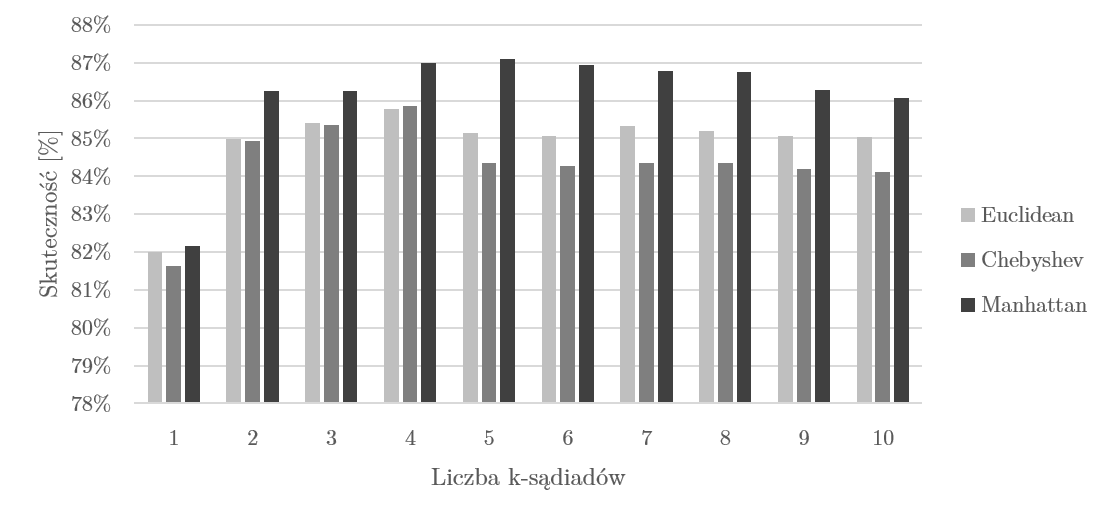
\includegraphics[width=1\textwidth]{{Wykresy/TF_10k.png}}
	\caption{}
\end{figure}

\section{Opis implementacji}
{\color{blue}
Należy tu zamieścić krótki i zwięzły opis zaprojektowanych klas oraz powiązań
między nimi. Powinien się tu również znaleźć diagram UML  (diagram klas)
prezentujący najistotniejsze elementy stworzonej aplikacji. Należy także
podać, w jakim języku programowania została stworzona aplikacja. }

\section{Materiały i metody}
{\color{blue}
W tym miejscu należy opisać, jak przeprowadzone zostały wszystkie badania,
których wyniki i dyskusja zamieszczane są w dalszych sekcjach. Opis ten
powinien być na tyle dokładny, aby osoba czytająca go potrafiła wszystkie
przeprowadzone badania samodzielnie powtórzyć w celu zweryfikowania ich
poprawności (a zatem m.in. należy zamieścić tu opis architektury sieci,
wartości współczynników użytych w kolejnych eksperymentach, sposób
inicjalizacji wag, metodę uczenia itp. oraz informacje o danych, na których
prowadzone były badania). Przy opisie należy odwoływać się i stosować do
opisanych w sekcji drugiej wzorów i oznaczeń, a także w jasny sposób opisać
cel konkretnego testu. Najlepiej byłoby wyraźnie wyszczególnić (ponumerować)
poszczególne eksperymenty tak, aby łatwo było się do nich odwoływać dalej.}

\section{Wyniki}
{\color{blue}
W tej sekcji należy zaprezentować, dla każdego przeprowadzonego eksperymentu,
kompletny zestaw wyników w postaci tabel, wykresów itp. Powinny być one tak
ponazywane, aby było wiadomo, do czego się odnoszą. Wszystkie tabele i wykresy
należy oczywiście opisać (opisać co jest na osiach, w kolumnach itd.) stosując
się do przyjętych wcześniej oznaczeń. Nie należy tu komentować i interpretować
wyników, gdyż miejsce na to jest w kolejnej sekcji. Tu również dobrze jest
wprowadzić oznaczenia (tabel, wykresów) aby móc się do nich odwoływać
poniżej.}

\section{Dyskusja}
{\color{blue}
Sekcja ta powinna zawierać dokładną interpretację uzyskanych wyników
eksperymentów wraz ze szczegółowymi wnioskami z nich płynącymi. Najcenniejsze
są, rzecz jasna, wnioski o charakterze uniwersalnym, które mogą być istotne
przy innych, podobnych zadaniach. Należy również omówić i wyjaśnić wszystkie
napotakane problemy (jeśli takie były). Każdy wniosek powinien mieć poparcie
we wcześniej przeprowadzonych eksperymentach (odwołania do konkretnych
wyników). Jest to jedna z najważniejszych sekcji tego sprawozdania, gdyż
prezentuje poziom zrozumienia badanego problemu.}
\section{Wnioski}
{\color{blue}W tej, przedostatniej, sekcji należy zamieścić podsumowanie
najważniejszych wniosków z sekcji poprzedniej. Najlepiej jest je po prostu
wypunktować. Znów, tak jak poprzednio, najistotniejsze są wnioski o
charakterze uniwersalnym.}


\begin{thebibliography}{0}
\end{thebibliography}
{\color{blue} 
Na końcu należy obowiązkowo podać cytowaną w sprawozdaniu
literaturę, z której grupa korzystała w trakcie prac nad zadaniem (przykład na
końcu szablonu)}
\end{document}
